% ------------------------------------------------------------------------ %
% !TEX encoding = UTF-8
% !TEX TS-program = pdflatex
% !TEX root = ../Project.tex
% !TEX spellcheck = en-EN
% ------------------------------------------------------------------------ %
%
% ------------------------------------------------------------------------ %
% 	CHAPTER TITLE
% ------------------------------------------------------------------------ %
%
\chapter{DB Design}
%
%
\section{Entity Relationship}
\par The ER diagram shows how information is organized in the database at an abstract level.
\begin{figure}[h]
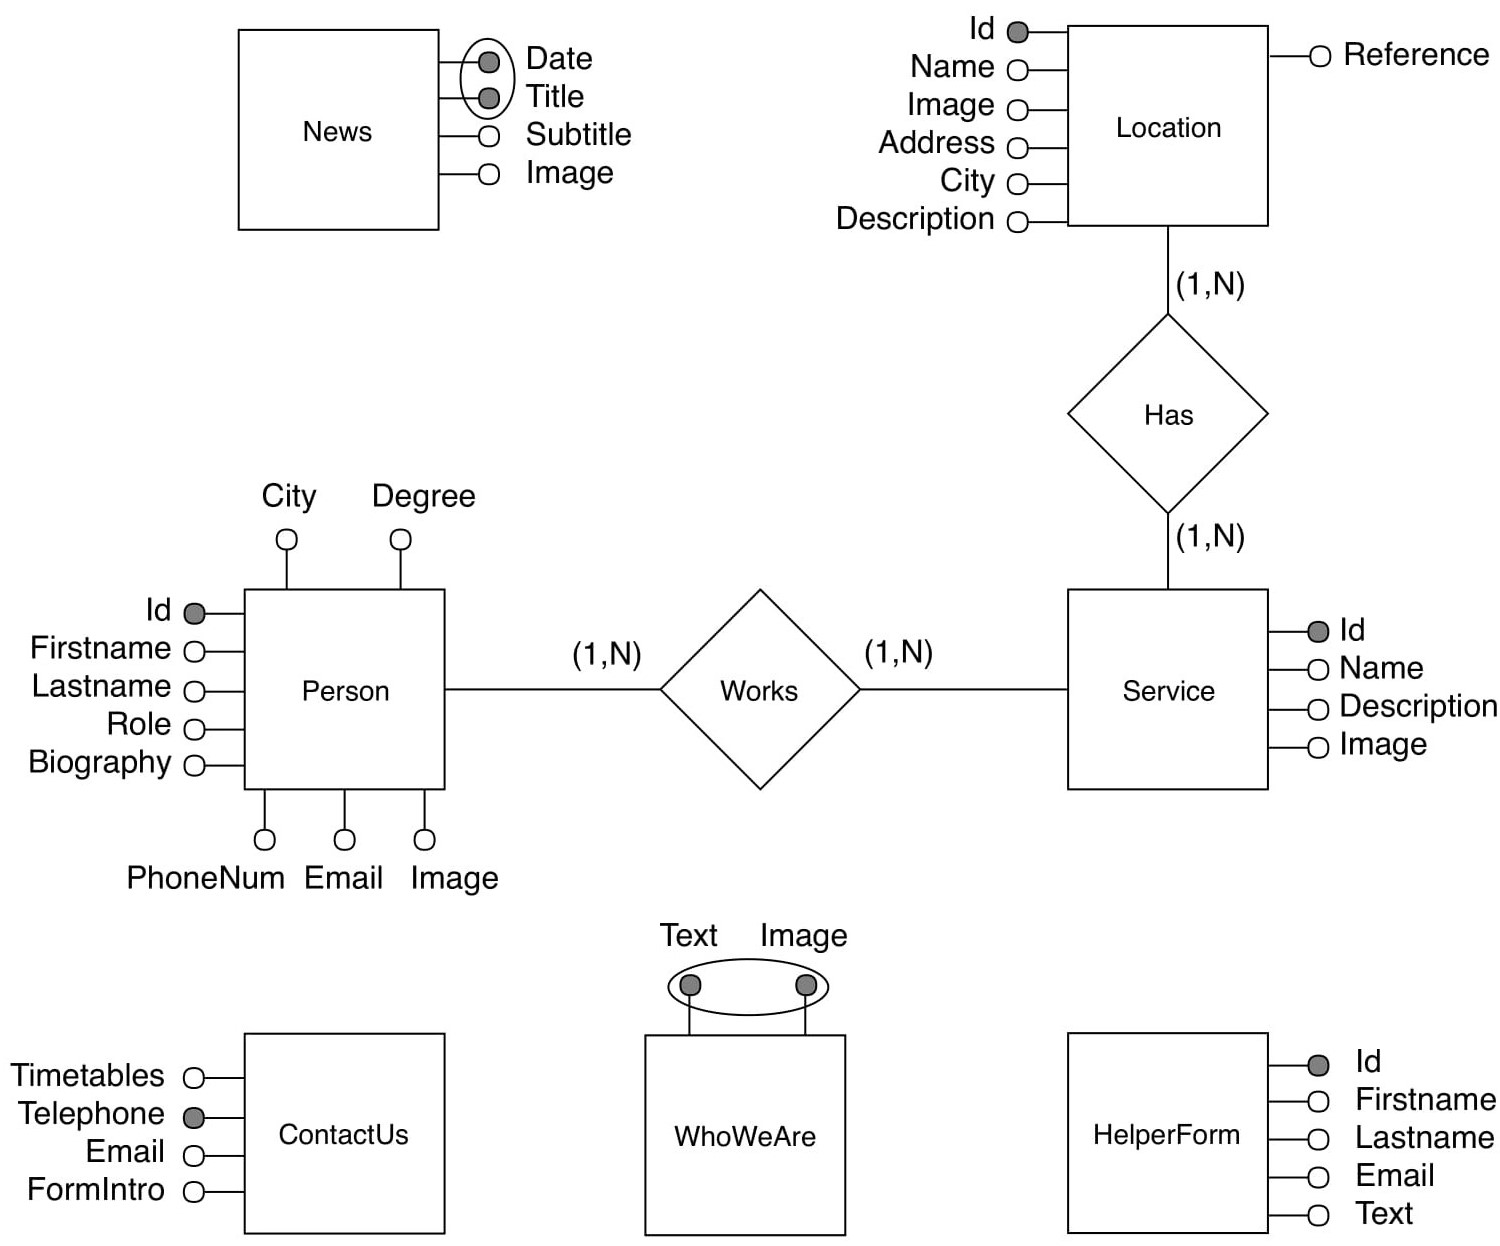
\includegraphics[width=1.2\textwidth, center]{MainMatter/images/ER.jpg}
\caption{Entity Relationship Diagram}
\label{fig:figure2}
\end{figure}
\newpage
%
\section{Tabular Structure}
\par The tabular structure represents how the DB is organized in a more concrete way, more similar to the final data structure used in the real database. 
\begin{figure}[h]
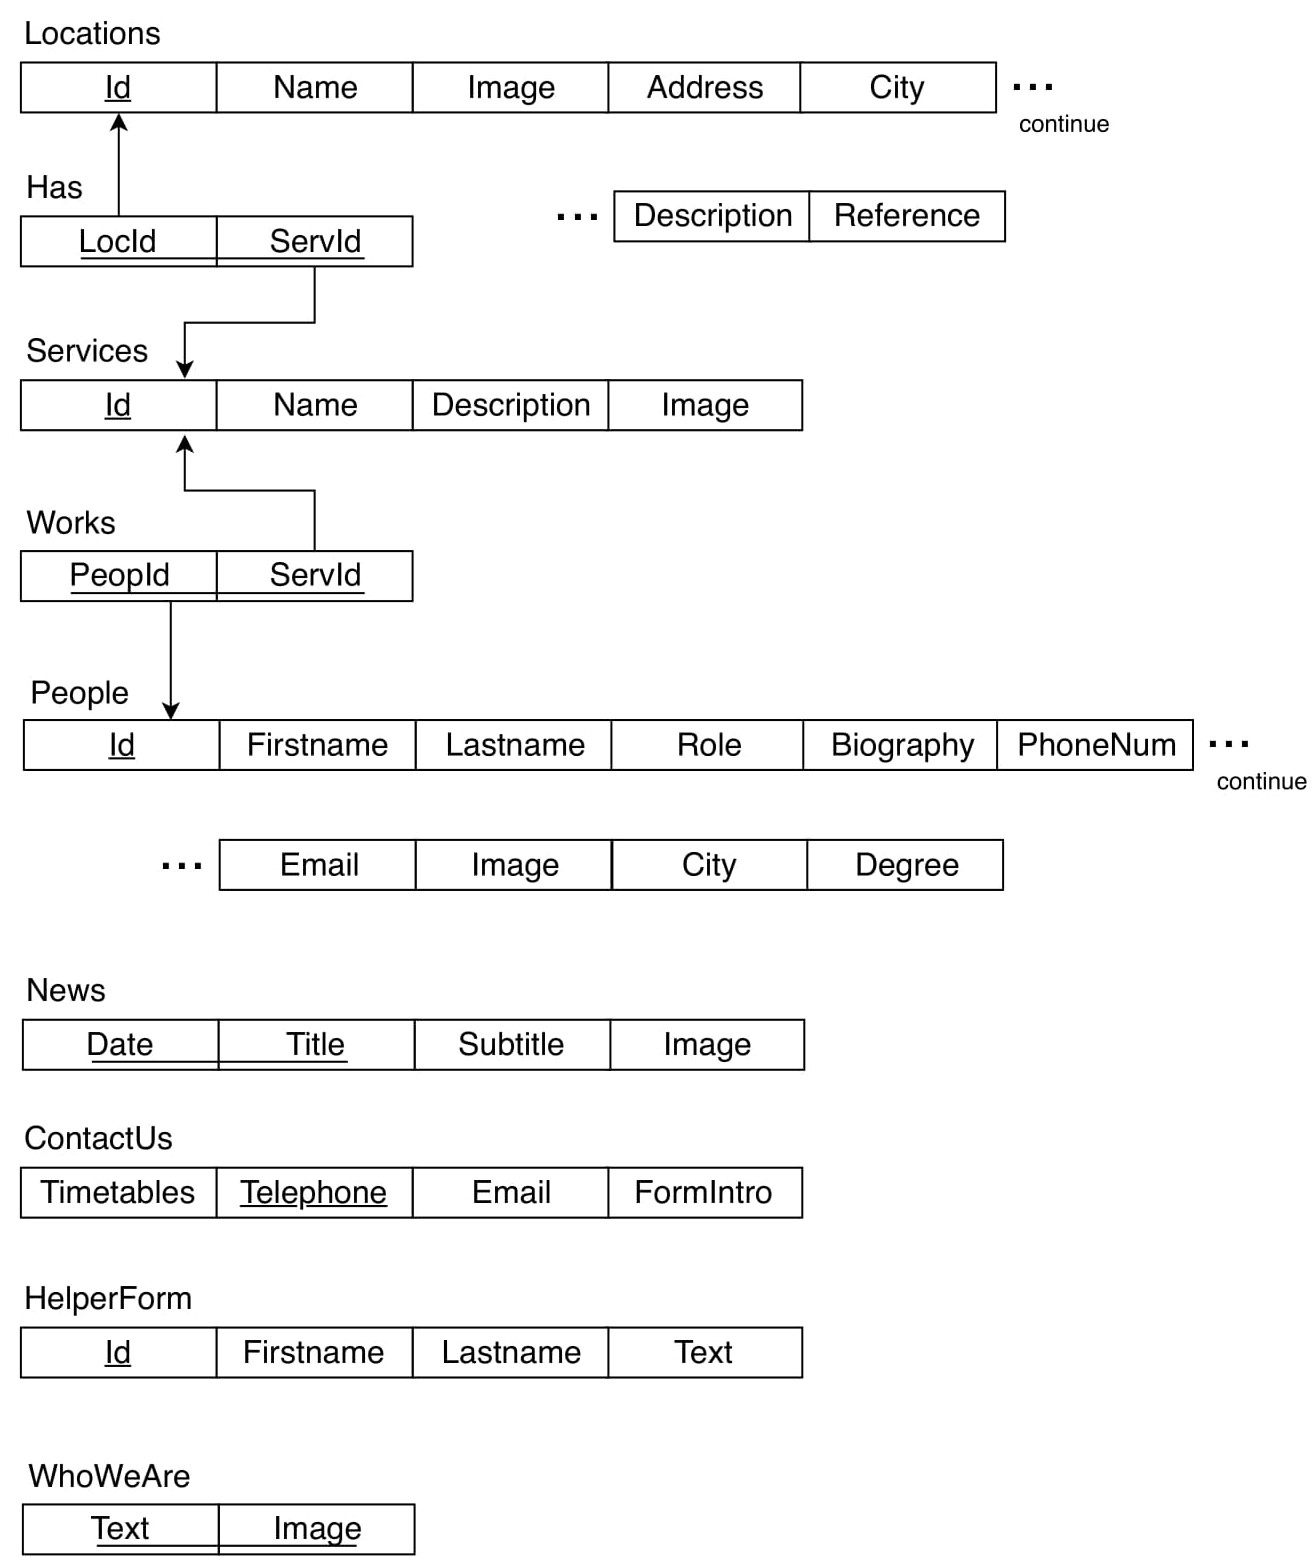
\includegraphics[width=1.2\textwidth, center]{MainMatter/images/DB.jpg}
\caption{Tabular Structure Diagram}
\label{fig:figure2}
\end{figure}
%
%
% -----------------------------END------------------------------------- %
